\documentclass[11pt,a4paper]{article}

\usepackage[T1]{fontenc}
\usepackage[utf8]{inputenc}
\usepackage[margin=1.1in]{geometry}
\usepackage{amsmath,amssymb,mathtools}
\usepackage{booktabs}
\usepackage{graphicx}
\usepackage[protrusion=true,expansion=false]{microtype}
\usepackage{enumitem}
\usepackage[dvipsnames]{xcolor}
\usepackage{tcolorbox}
\usepackage{tikz}
\usepackage{float}
\usepackage{siunitx}
\usepackage{caption}
\usepackage[hidelinks]{hyperref}
\usepackage{cleveref}

\tcbuselibrary{skins,breakable}
\usetikzlibrary{arrows.meta,decorations.pathmorphing,positioning}

% ---- palette: the project's own line-loading heat scale ------------------
\definecolor{anchorclr}{HTML}{B8730B}   % amber  - the physical object
\definecolor{buildclr}{HTML}{12768F}    % teal   - the formal machinery
\definecolor{teachclr}{HTML}{5B7C1F}    % olive  - say it back
\definecolor{warnclr}{HTML}{C0362A}     % red    - watch out
\definecolor{inkclr}{HTML}{0D2233}
\definecolor{softbg}{HTML}{F4F7F8}

% ---- boxes ---------------------------------------------------------------
\newtcolorbox{anchor}[1][]{
  breakable, enhanced, colback=anchorclr!6, colframe=anchorclr,
  boxrule=0pt, leftrule=3pt, arc=1pt, left=8pt, right=8pt, top=7pt, bottom=7pt,
  fonttitle=\bfseries\sffamily, coltitle=anchorclr,
  title={ANCHOR \textemdash\ the object}, #1}

\newtcolorbox{build}[1][]{
  breakable, enhanced, colback=buildclr!5, colframe=buildclr,
  boxrule=0pt, leftrule=3pt, arc=1pt, left=8pt, right=8pt, top=7pt, bottom=7pt,
  fonttitle=\bfseries\sffamily, coltitle=buildclr,
  title={BUILD \textemdash\ the notation}, #1}

\newtcolorbox{teach}[1][]{
  breakable, enhanced, colback=teachclr!6, colframe=teachclr,
  boxrule=0pt, leftrule=3pt, arc=1pt, left=8pt, right=8pt, top=7pt, bottom=7pt,
  fonttitle=\bfseries\sffamily, coltitle=teachclr,
  title={TEACH IT BACK}, #1}

\newtcolorbox{watch}[1][]{
  breakable, enhanced, colback=warnclr!5, colframe=warnclr,
  boxrule=0pt, leftrule=3pt, arc=1pt, left=8pt, right=8pt, top=7pt, bottom=7pt,
  fonttitle=\bfseries\sffamily, coltitle=warnclr,
  title={THE CATCH}, #1}

\newcommand{\okina}{\textquoteleft}
\newcommand{\R}{\mathbb{R}}
\newcommand{\E}{\mathbb{E}}
\newcommand{\Prob}{\mathbb{P}}
\newcommand{\CV}{\operatorname{CV}}
\newcommand{\VOLL}{\mathrm{VOLL}}

\sisetup{detect-weight=true, group-separator={,}}
\captionsetup{font=small,labelfont=bf}
\setlist{itemsep=0.25em,topsep=0.4em}

\title{\bfseries Two Fences\\[0.3em]
\large A Reader's Companion to\\
\emph{Radial and Angular Risk in Stochastic DC Optimal Power Flow}}
\author{Written for Pascual}
\date{13 September 2026}

\begin{document}
\maketitle

\begin{center}
\begin{minipage}{0.86\textwidth}
\small\itshape
This is the same paper you already have, rebuilt out of objects you can hold.
Every proposition in the formal paper appears here in the same order and with
the same number, so you can read the two side by side. Nothing is watered
down---the rigour is identical. Only the packaging changed.
\end{minipage}
\end{center}

\vspace{1em}
\tableofcontents
\newpage

% =========================================================================
\section{First: how to read a paper like this}
% =========================================================================

The formal paper is written in a house style that mathematicians use because it
compresses well, not because it is trying to be difficult. Here is the whole
vocabulary in one table.

\begin{center}
\small
\begin{tabular}{@{}p{0.20\textwidth}p{0.74\textwidth}@{}}
\toprule
\textbf{Word} & \textbf{What it actually means} \\
\midrule
\textbf{Definition} & ``Here is a name I am about to reuse fifty times. Pin it down now so I never have to re-explain it.'' Carries no claim---you cannot disagree with a definition, only find it useless. \\[0.4em]
\textbf{Proposition} & A claim that is true, and here is why. The workhorse. \\[0.4em]
\textbf{Theorem} & A proposition the author thinks is the important one. Same logical status; more self-importance. \\[0.4em]
\textbf{Lemma} & A small true thing proved only because a bigger proof needs it. A stepping stone. \\[0.4em]
\textbf{Corollary} & ``And therefore, almost for free, this too.'' It falls out of the thing just proved with barely any extra work. \\[0.4em]
\textbf{Remark} & A comment. Often the most useful part, because it is where the author admits what worried them. \\[0.4em]
\textbf{Proof} & The argument. Ends with $\square$, which just means \emph{done}. \\[0.4em]
\textbf{iff} & ``if and only if''---the claim runs in both directions. Not a typo. \\
\bottomrule
\end{tabular}
\end{center}

\paragraph{How to actually read one.}
Not front to back. Do this instead:

\begin{enumerate}[label=\textbf{\arabic*.}]
\item Read the abstract. Then read the conclusion. Now you know where it lands.
\item Read every \textbf{Definition} and the \emph{statement} of every
      \textbf{Proposition}, skipping all proofs. That is the whole skeleton, and
      it is usually four pages, not eighteen.
\item Only now go back for the proofs, and only for the results you doubt.
\end{enumerate}

A proof is not there to convince you the author is clever. It is there so that
if you \emph{don't} believe the claim, you have somewhere to push.

% =========================================================================
\section{The one picture that carries the whole paper}\label{sec:picture}
% =========================================================================

If you keep one thing from this document, keep this.

\begin{anchor}
You are standing in an open field at a spot marked \textbf{zero}---no
neighbourhood on the island is asking for any power at all.

Now demand starts to grow, and you \textbf{walk}.

\begin{itemize}
\item \textbf{How far you walk} = how much total power the island is asking
      for. A hundred metres out might be \SI{600}{\mega\watt}; four hundred
      metres out might be \SI{1100}{\mega\watt}.
\item \textbf{Which way you face} = the \emph{mix}. Walking north-east might
      mean ``Honolulu wants a lot and Waianae wants a little.'' Walking due
      south might mean the opposite.
\end{itemize}

Two fences are drawn on this field, and they are \textbf{not the same shape}.

\medskip
\textbf{The inner fence is round.} It sits about \SI{585}{\mega\watt} out in
every direction. Cross it and some transmission line somewhere hits its limit.
This is the \emph{congestion} fence.

\textbf{The outer fence is lumpy.} In some headings it sits \SI{1496}{\mega\watt}
out; in others it comes in as close as \SI{409}{\mega\watt}. Cross it and the
grid physically cannot deliver---you have to switch customers off. This is the
\emph{adequacy} fence.
\end{anchor}

\begin{figure}[H]
\centering
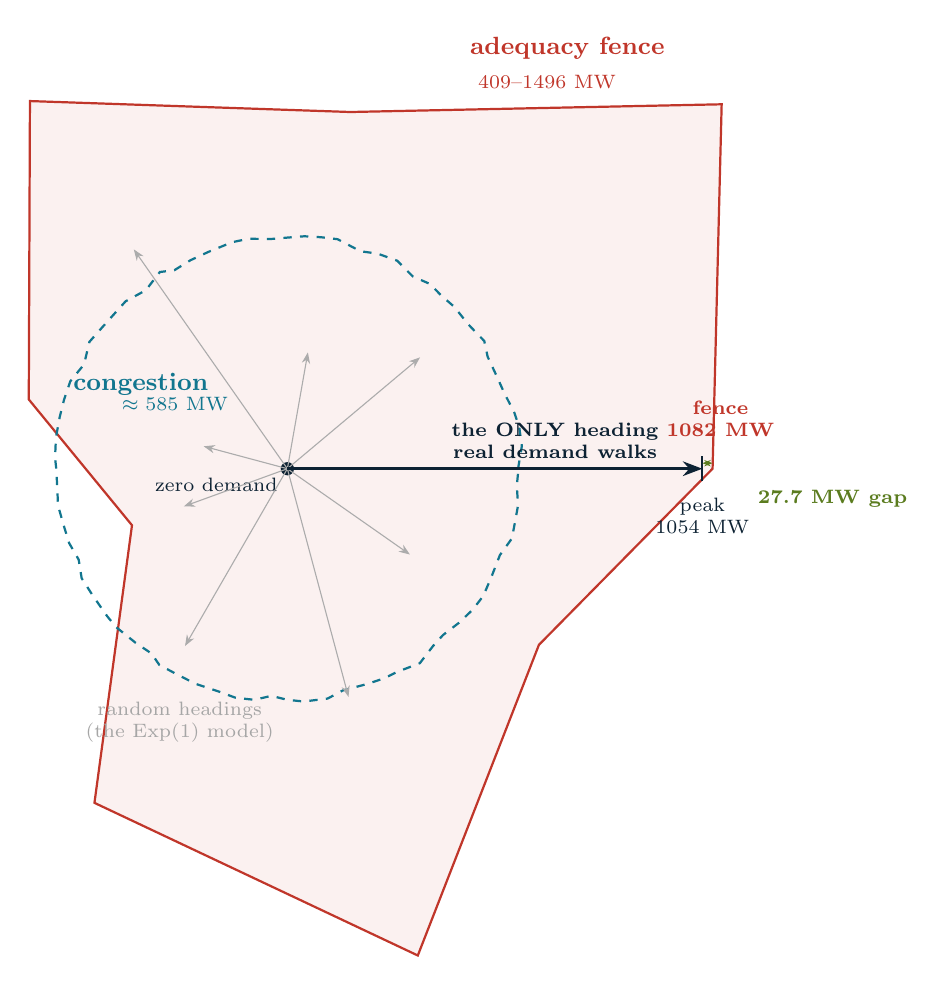
\begin{tikzpicture}[scale=1.0]

% --- the adequacy fence: an irregular polygon (it really is a polyhedron) ---
\draw[thick, warnclr, fill=warnclr!7]
  (0:5.4) -- (40:7.2) -- (80:4.6) -- (125:5.7) -- (165:3.4)
  -- (200:2.1) -- (240:4.9) -- (285:6.4) -- (325:3.9) -- cycle;

% --- the congestion fence: a gently wobbly near-circle ---------------------
\draw[thick, buildclr, dashed,
      decorate, decoration={random steps, segment length=7pt, amplitude=1.4pt}]
  (0,0) circle (2.93);

% --- origin ---------------------------------------------------------------
\fill[inkclr] (0,0) circle (2.4pt);
\node[below left, font=\scriptsize, inkclr] at (0,0) {zero demand};

% --- scattered random headings (the exponential model) --------------------
\foreach \a/\r in {40/2.2, 80/1.5, 125/3.4, 165/1.1, 200/1.4, 240/2.6, 285/3.0, 325/1.9}
  \draw[-{Stealth[length=4pt]}, gray!65, thin] (0,0) -- (\a:\r);

% --- the one heading real demand ever walks -------------------------------
\draw[-{Stealth[length=7pt]}, very thick, inkclr] (0,0) -- (0:5.27);
\draw[inkclr, thick] (0:5.27) ++(0,-0.16) -- ++(0,0.32);
\node[font=\scriptsize\bfseries, inkclr, above, align=center]
  at (0:3.4) {the ONLY heading\\real demand walks};

% Peak and fence ticks. These sit only 0.13cm apart radially, so the labels
% are pushed apart VERTICALLY -- one below the axis, one above -- rather than
% stacked on top of each other at the polygon vertex.
\node[font=\scriptsize, inkclr, align=center, anchor=north]
  at ([yshift=-7pt] 0:5.27) {peak\\1054 MW};
\node[font=\scriptsize\bfseries, warnclr, align=center, anchor=south]
  at ([yshift=8pt] 0:5.5) {fence\\1082 MW};
\draw[{Stealth[length=3pt]}-{Stealth[length=3pt]}, teachclr, semithick]
  ([yshift=2pt] 0:5.27) -- ([yshift=2pt] 0:5.4);
\node[font=\scriptsize\bfseries, teachclr, anchor=west]
  at ([xshift=10pt, yshift=-11pt] 0:5.5) {27.7 MW gap};

% --- labels ---------------------------------------------------------------
\node[buildclr, font=\small\bfseries] at (150:2.15) {congestion};
\node[buildclr, font=\scriptsize] at (150:1.65) {$\approx585$ MW};
\node[warnclr, font=\small\bfseries, above] at (55:6.2) {adequacy fence};
\node[warnclr, font=\scriptsize, above] at (55:5.75) {409--1496 MW};
\node[gray!70, font=\scriptsize, align=center] at (247:3.5)
  {random headings\\(the Exp(1) model)};

\end{tikzpicture}
\caption{The two fences. Distance from the centre is \emph{how much} power the
island wants; the direction you face is \emph{which neighbourhoods} want it.
Congestion is a near-circle---it barely cares about direction. Adequacy is a
lumpy polygon---it cares enormously. Real O\okina ahu demand only ever walks one
heading (bold), stopping \SI{27.7}{\mega\watt} short of the fence. Note the
heading near the bottom-left where the lumpy fence dips \emph{inside} the round
one: in a few unlucky mixes the grid runs out of delivery before the network is
even fully stressed. This is a two-dimensional shadow of an eight-dimensional
picture---there is one axis per load bus---but every feature drawn is real.}
\label{fig:fences}
\end{figure}

\medskip
Everything else in the paper is a consequence of \Cref{fig:fences}:

\begin{center}
\small
\begin{tabular}{@{}p{0.42\textwidth}p{0.52\textwidth}@{}}
\toprule
\textbf{What the picture shows} & \textbf{Which result says it} \\
\midrule
The servable region has no holes: walk out along a heading and you are fine, fine, fine, then never fine again. & Proposition 4.1 \\[0.35em]
Whether you shed depends on \emph{which way you face}, because the outer fence is lumpy. & Corollary 4.2 \\[0.35em]
Whether you congest barely depends on facing at all, because the inner fence is round. & Proposition 4.5 \\[0.35em]
Real demand always walks one heading, and the fence on that heading is \SI{1082}{\mega\watt} while demand tops out at \SI{1054}{\mega\watt}. & Theorem 4.6 \\
\bottomrule
\end{tabular}
\end{center}

% =========================================================================
\section{The machine (paper \S2)}
% =========================================================================

\subsection{The rig}

\begin{anchor}
A plumbing rig bolted to a wall.

\begin{itemize}
\item \textbf{Pumps} = generators. Each has a maximum it can push and a price
      per litre.
\item \textbf{Pipes} = transmission lines. Each has a maximum it can carry.
\item \textbf{Taps} = the neighbourhoods. Each is opened to some position; that
      is the demand.
\item \textbf{Pressure} = voltage phase angle. Water runs from high pressure to
      low, and how much runs down a pipe is set by the pressure \emph{drop}
      across it. You never choose the flows directly---you choose the
      pressures, and the flows follow.
\end{itemize}

Your job: open the cheapest pumps needed to satisfy every tap, without
overloading any pipe.
\end{anchor}

\begin{build}
That is the linear program labelled (1) in the paper. Piece by piece:

\smallskip
\begin{tabular}{@{}llp{0.38\textwidth}@{}}
\toprule
\textbf{Symbol} & \textbf{Object} & \textbf{Its job} \\
\midrule
$P_g$      & how hard \textbf{pump} $g$ is running & what you choose \\
$p^{\max}_g$ & the pump's \textbf{rating plate} & you cannot exceed it \\
$c_g$      & the \textbf{price tag} on that pump & \si{\per\mega\watt\hour} \\
$\theta_i$ & \textbf{pressure} at junction $i$ & what you really choose \\
$F_\ell$   & \textbf{flow} down pipe $\ell$ & follows from the pressures \\
$\bar F_\ell$ & the pipe's \textbf{diameter rating} & flow can't exceed it \\
$D_i$      & how far \textbf{tap} $i$ is opened & the random part \\
$S_i$      & water that \textbf{spills out the drain} at tap $i$ & unserved demand \\
\bottomrule
\end{tabular}

\smallskip
And the objective, equation (1a):
\[
\min \;\; \underbrace{\sum_g c_g P_g}_{\text{the fuel bill}}
\;+\; \underbrace{\VOLL \sum_i S_i}_{\text{the fine for spilling}}
\]
\end{build}

\subsection{Proposition 2.4 --- the rig can never break}

The claim: \emph{no matter how the taps are set, there is always a valid setting
of the rig.}

\begin{anchor}
Turn every pump \textbf{off}. Let every tap spill entirely down its drain.

Nothing is being delivered, and the fine is enormous---but look at the
rig: no pump exceeds its plate (they're off), no pipe exceeds its rating
(nothing is flowing), and the books balance at every junction (zero in, zero
out). It is a \emph{terrible} answer. It is a \emph{valid} answer.
\end{anchor}

That is the entire proof. In this kind of mathematics, to prove ``a valid
setting exists'' you do not reason about all possible settings---you
\textbf{point at one}. Finding an ugly one is completely legitimate.

\begin{watch}
Why bother proving something so obvious? Because without it the whole study is
built on sand.

If the rig could break, then a run where the solver returns
\texttt{INFEASIBLE} is \emph{ambiguous}: did the island genuinely run out of
power, or did the solver just trip over a rounding error? You'd be counting two
different things in the same bucket. \textbf{Proposition 2.4 guarantees the
solver never has an excuse}, so every failure that appears is a real one, and
it arrives as a number of megawatts rather than a shrug.
\end{watch}

\subsection{Proposition 2.5 --- how big must the fine be?}

Making the rig unbreakable creates a new problem: now it can spill \emph{by
choice}. If the fine is low, the optimiser will cheerfully cut off a
neighbourhood to avoid firing an expensive pump---and you would record that as
a blackout when it was really a purchasing decision.

So: how high must the fine be?

\begin{anchor}
The obvious guess is \textbf{``higher than the most expensive pump.''} That
guess is wrong, and the reason is worth holding onto.

Picture a tap at the far end of a pipe that is already completely full. That
neighbourhood cannot get one more litre \emph{at any price}, because the pipe
is the constraint, not the pumps. If you could somehow teleport one litre in,
what would it be worth there? Far more than the priciest pump charges---because
the scarcity is the pipe, and the pipe is not for sale.

In our own data this is not hypothetical: the Part 4 study recorded a price of
\SI{381}{\per\mega\watt\hour} at a bottled-up bus, against a most expensive
generator of \SI{237.97}{\per\mega\watt\hour}.
\end{anchor}

\begin{build}
The quantity you must beat is $\lambda^\circ_i$---the \textbf{value of one more
megawatt at bus $i$}, which economists call the locational marginal price and
mathematicians call a \emph{dual}. The condition is equation (9):
\[
\VOLL \;>\; \max_i \lambda^\circ_i .
\]
We set $\VOLL = \SI{10000}{\per\mega\watt\hour}$---about $42\times$ the
costliest generator---and then \textbf{checked it held} on \num{6000}
replications. Every time the model shed load, an independent test confirmed
that serving that demand was genuinely impossible. No exceptions.
\end{build}

\paragraph{The one piece of machinery in the proof.}
The proof leans on a shape, so let me give you the shape.

\begin{anchor}
Let $V(u)$ be \emph{the cheapest possible fuel bill to serve demand $u$}. Plot
it. It is \textbf{bowl-shaped}: as you demand more, cost rises, and it rises
ever more steeply, because you are climbing the merit order into worse and
worse pumps.

Now take a \textbf{straight ruler} and slide it up underneath the bowl until it
just touches at one point. The ruler lies below the curve everywhere and
touches it once.

That ruler is a \textbf{subgradient}. Its slope is $\lambda^\circ$---the price
of one more megawatt right there.
\end{anchor}

The proof then says, in one line: shedding a megawatt saves you at most what the
ruler's slope promises, and costs you $\VOLL$. If $\VOLL$ beats every ruler
slope, shedding is always a losing trade. Hence it only ever happens when
serving the demand was impossible to begin with. $\square$

\begin{teach}
Explain to a friend, using the full-pipe picture and no symbols, why ``set the
penalty higher than the most expensive generator'' is not a safe rule.
\end{teach}

% =========================================================================
\section{Rolling the dice (paper \S3)}
% =========================================================================

Three ways to decide how far the taps get opened.

\begin{center}
\small
\begin{tabular}{@{}llp{0.50\textwidth}@{}}
\toprule
& \textbf{Name in the paper} & \textbf{What it does} \\
\midrule
\textbf{A} & independent $\mathrm{Exp}(1)$ & Every tap rolls its own die, nobody
coordinates. The assignment's starting point. \\[0.35em]
\textbf{B} & common-shock mixture & One island-wide shock plus private noise at
each tap. Closer to physics: one weather system. \\[0.35em]
\textbf{C} & empirical resampling & No invented distribution at all. Pull a real
hour out of the \num{8760} on record. \\
\bottomrule
\end{tabular}
\end{center}

\subsection{Proposition 3.4 --- the geometry of diversification}

This is the result I most want you to actually \emph{see}, because it looks like
algebra and is really a picture.

Each tap has $\CV = 1$ (as volatile as it is large). But the \emph{island total}
does not. The paper says
\[
\CV(\text{total}) \;=\; \frac{\sqrt{\sum_i \mu_i^2}}{\sum_i \mu_i}
\;=\; \frac{\lVert \mu \rVert_2}{\lVert \mu \rVert_1}.
\]

\begin{anchor}
Two ways to measure how far you have travelled across a city.

\begin{itemize}
\item $\lVert\mu\rVert_1$ --- \textbf{the walk.} You go three blocks east, then
      four blocks north. Distance travelled: $3 + 4 = 7$ blocks. Add up every
      leg.
\item $\lVert\mu\rVert_2$ --- \textbf{the helicopter.} Straight line from start
      to finish: $\sqrt{3^2+4^2} = 5$ blocks.
\end{itemize}

The ratio $\lVert\mu\rVert_2 / \lVert\mu\rVert_1 = 5/7$ is a measure of
\textbf{how many different directions your trip used}.
\end{anchor}

\begin{build}
Now read the two extremes off the picture.

\smallskip
\begin{tabular}{@{}p{0.31\textwidth}p{0.30\textwidth}p{0.30\textwidth}@{}}
\toprule
& \textbf{All load at one bus} & \textbf{Load spread evenly over $n$} \\
\midrule
The trip & one straight leg & a long zigzag \\
Helicopter vs walk & identical & helicopter much shorter \\
Ratio & $1$ & $1/\sqrt{n}$ \\
Meaning & no cancellation & maximum cancellation \\
\bottomrule
\end{tabular}

\smallskip
So the bound in the paper,
\[
\frac{1}{\sqrt{n}} \;\le\; \CV(\text{total}) \;\le\; 1,
\]
is just the statement that \textbf{the helicopter never beats the walk, and
never loses by more than $\sqrt{n}$}. That is the Cauchy--Schwarz inequality,
and that is all it is.
\end{build}

\begin{watch}
Read the consequence carefully, because it is the opposite of the usual
intuition.

The volatility of the island total is \textbf{not} a property of the
distribution you assumed. It is a property of \textbf{how concentrated the load
is}. O\okina ahu gets $\CV = 0.534$ and IEEE-14 gets $0.444$ from the
\emph{identical} demand model---because two O\okina ahu buses carry
$\SI{72.4}{\percent}$ of the island, so there is less for the randomness to
cancel against.

Concentrated load diversifies less. Geography, not statistics.
\end{watch}

\subsection{Proposition 3.6 --- the knob that does two things at once}

Model B has a knob $w$: how much of each tap's behaviour comes from the shared
island-wide shock rather than its own private noise.

\begin{anchor}
Rolling dice for each tap's demand.

\begin{itemize}
\item $w = 0$: every tap rolls \textbf{its own} die. Independent.
\item $w = 1$: one die is rolled \textbf{once} and every tap copies it. Perfect
      lockstep.
\item $w = 0.7$: each tap's number is $70\%$ the shared die, $30\%$ its own.
\end{itemize}
\end{anchor}

\begin{build}
The paper derives, for any two taps $i \ne j$:
\[
\CV(D_i) = \sqrt{w^2 + (1-w)^2},
\qquad
\operatorname{Corr}(D_i, D_j) = \frac{w^2}{w^2 + (1-w)^2}.
\]
At the value used, $w = 0.7$: correlation $= 0.845$, nodal $\CV = 0.762$.
\end{build}

\begin{watch}
Two things here caught us out, and both are stated in the paper as corrections.

\smallskip
\textbf{One: $w$ is not the correlation.} Setting $w = 0.7$ gives correlation
$0.845$, not $0.7$. It is a \emph{mixing weight}---how much of the recipe comes
from the shared jar---and the correlation it produces is a different number.
The earlier write-up called it a correlation. That was wrong, and it is
corrected.

\smallskip
\textbf{Two: turning the knob moves two things at once.} Look at the $\CV$
formula as $w$ goes $0 \to 1$:
\[
1 \;\longrightarrow\; \tfrac{1}{\sqrt2} \approx 0.707 \;\longrightarrow\; 1 .
\]
It \textbf{dips in the middle}. Averaging two independent dice is steadier than
either one alone---the same reason two coin flips vary less than one. So moving
$w$ off zero \emph{raises} correlation and \emph{lowers} each tap's volatility,
simultaneously.

That means Model B is \textbf{not a clean experiment about correlation}. It is a
joint sensitivity, and the paper labels it as one rather than pretending
otherwise.
\end{watch}

% =========================================================================
\section{The geometry of failure (paper \S4)}
% =========================================================================

Now back to \Cref{fig:fences}, with the results attached.

\subsection{Proposition 4.1 --- no holes}

The claim: walk out along a fixed heading, and the stretch you can serve is one
unbroken run from zero out to the fence. You never get a gap---servable, then
not, then servable again.

\begin{anchor}
Suppose you have a working setup at full demand: pumps at certain levels, water
moving down the pipes, every tap satisfied.

Now \textbf{shrink the whole thing by the same factor}---a scale model. Every
pump at $60\%$, every flow at $60\%$, every tap at $60\%$.

Check the rig: every pump is running \emph{lower} than before, so still under
its plate. Every pipe carries \emph{less}, so still under its rating. And the
books still balance, because halving everything on both sides of an equation
keeps it true.
\end{anchor}

That is the proof. Every constraint in the model is a straight-line
relationship, and every limit is a ceiling---so scaling a valid answer
\emph{down} can never break it. Hence the servable stretch runs from $0$ out to
some furthest point, with nothing missing in between. The paper calls that
furthest point $T^\star(\sigma)$: \textbf{how far the fence is, on the heading
you're facing}.

\subsection{Corollary 4.2 --- adequacy is about which way you face}

Once you have the fence distance $T^\star$, the entire adequacy question reduces
to one comparison:

\begin{center}
\begin{tcolorbox}[colback=softbg,colframe=inkclr,boxrule=0.6pt,arc=1pt,width=0.82\textwidth]
\centering
\textbf{You must shed load} $\iff$ \textbf{how far you walked} $>$
\textbf{how far the fence is on your heading}
\[
\lVert D \rVert_1 \;>\; T^\star\!\left(\frac{D}{\lVert D\rVert_1}\right)
\]
\end{tcolorbox}
\end{center}

The bar you must clear is \textbf{not a fixed number}. It moves depending on
which way you face. That is what ``adequacy is angular'' means, and the numbers
show how much it moves:

\begin{center}
\small
\begin{tabular}{@{}lr@{}}
\toprule
\textbf{Fence distance $T^\star$, over random headings} & \textbf{MW} \\
\midrule
Worst heading found & 409 \\
$1$st percentile & 592 \\
Median heading & 1028 \\
$99$th percentile & 1238 \\
Best heading found & 1496 \\
\midrule
\textbf{The heading real demand actually walks} & \textbf{1082} \\
\bottomrule
\end{tabular}
\end{center}

Read the last two lines together. The real heading is a \emph{comparatively
lucky} one: $\SI{64.7}{\percent}$ of random headings have their fence closer in
than the real one does.

\subsection{Proposition 4.5 --- and here is where I was wrong}

\begin{watch}
I want you to see this one as a mistake being caught, because that is what it
was.

\textbf{My guess:} congestion would also be angular. The reasoning felt
airtight---a line gets full when power has to \emph{cross} it, and whether power
crosses it depends on \emph{where} the demand sits. So the congestion fence
should be lumpy too.

\textbf{The test that killed it.} Sort every scenario by total demand into
bands. Then, \emph{within a single band}, compare the two demand models. If
congestion were about direction, the models would disagree inside a band,
because they face different ways. If it were about magnitude, they would agree,
because inside a band they walked the same distance.

\smallskip
\begin{tabular}{@{}lcc@{}}
\toprule
Total demand band & Model A congests & Model C congests \\
\midrule
600--700 MW & 93.4\% & 100\% \\
700--800 MW & 99.7\% & 100\% \\
800--900 MW & 100\%\phantom{.0} & 100\% \\
\bottomrule
\end{tabular}

\smallskip
\textbf{They agree.} Conditioning on distance walked wipes out nearly all the
difference between two radically different demand models. Congestion is
\emph{radial}---a threshold on how far you walked, roughly regardless of
heading.
\end{watch}

The clinching number: one single threshold, $t_c = \SI{585}{\mega\watt}$,
reproduces \emph{both} models' congestion rates.

\begin{center}
\small
\begin{tabular}{@{}lcc r@{}}
\toprule
& Predicted by ``walked past 585 MW?'' & Actually observed & Error \\
\midrule
Model A (exponential) & 59.0\% & 58.4\% & $0.6$ pts \\
Model C (real hours)  & 92.0\% & 92.5\% & $-0.5$ pts \\
\bottomrule
\end{tabular}
\end{center}

Two models whose congestion rates differ by \textbf{34 percentage points}, both
predicted to within \textbf{half a point} by one number. The 34-point gap was
never about direction at all---it is just that the exponential spends
$\SI{42.8}{\percent}$ of its time loafing around \emph{inside} the round fence,
while real demand is almost always outside it.

\begin{teach}
In one sentence, no symbols: why does sorting scenarios by total demand first,
and only then comparing the two models, settle whether a failure mode is about
distance or about direction?
\end{teach}

\subsection{Theorem 4.6 --- why the real island never sheds}

\begin{anchor}
Go back to the bold arrow in \Cref{fig:fences}.

Real O\okina ahu demand, as we model it, \textbf{always walks the exact same
heading}. The neighbourhood shares never change---Honolulu is always
$\SI{39.9}{\percent}$ of the island, Ewa-Central always $\SI{32.5}{\percent}$.
Only the \emph{distance} varies, hour to hour.

So the question collapses. There is only one fence distance that matters:
\SI{1082}{\mega\watt}, the fence on that one heading. And in \num{8760} recorded
hours, the furthest the island ever walked was \SI{1054.3}{\mega\watt}.
\end{anchor}

\begin{center}
\begin{tcolorbox}[colback=warnclr!6,colframe=warnclr,boxrule=0pt,leftrule=3pt,
                  arc=1pt,width=0.88\textwidth]
\centering
\SI{1082.0}{\mega\watt} fence $-$ \SI{1054.3}{\mega\watt} peak
$=$ \textbf{\SI{27.7}{\mega\watt} of margin} $=$ \textbf{2.63\%}
\end{tcolorbox}
\end{center}

Zero shedding is a real result. But it is a \emph{2.63\% margin}, not a
comfortable one---and that is the number worth quoting, not the zero.

\begin{watch}
Compare the margin you would quote if you only looked at the nameplate on the
generators:
\[
\frac{\SI{1508}{\mega\watt} - \SI{1054}{\mega\watt}}{\SI{1054}{\mega\watt}}
= \SI{43}{\percent} \qquad\text{versus}\qquad \SI{2.63}{\percent}.
\]
The gap is \SI{426}{\mega\watt} of generation that exists but sits
\textbf{stranded behind one \SI{400}{\mega\watt} corridor}---Ewa-West to
Ewa-Central, which under real load runs at $\SI{97.7}{\percent}$ of its rating
on average.

A megawatt you cannot move is not capacity.
\end{watch}

% =========================================================================
\section{Counting carefully (paper \S5)}
% =========================================================================

\subsection{Error bars, and why the textbook formula fails here}

We ran \num{10000} scenarios and got $\SI{41.58}{\percent}$ shedding. How much of
that last digit is real?

\begin{anchor}
It is a coin-flip problem. Flip \num{10000} times, count heads, and ask how far
the true rate could be from what you saw. At this sample size the answer is
about $\pm 1$ percentage point.
\end{anchor}

\begin{watch}
Now the case that breaks the standard formula. Model C shed load in
\textbf{zero} of \num{10000} scenarios.

The textbook interval is $\hat p \pm z\sqrt{\hat p (1-\hat p)/N}$. Put
$\hat p = 0$ in and everything collapses: the interval is
$[0, 0]$. That says \textbf{``this can never happen''} on the strength of
\num{10000} trials---which is obvious nonsense. A one-in-a-million event would
also show up zero times in \num{10000} draws.

The \textbf{Wilson interval} (equation 11) handles the edge properly and returns
$[0,\; \SI{0.038}{\percent}]$. In words: \emph{``we saw none, and the true rate
is below about 1 in 2{,}600---but it is not necessarily zero.''}

That is why the paper reports zero shedding \emph{and} the
\SI{2.63}{\percent} margin. The zero is what we measured; the margin is what we
know.
\end{watch}

\subsection{Proposition 5.2 --- when the solver is picking, not the physics}

\begin{anchor}
Two workers, identical in every way, paid exactly the same wage. You need
\SI{100}{\mega\watt} of work done.

Any split works: $100/0$, $50/50$, $73/27$. The \textbf{total} is pinned by the
job. \textbf{Who does what} is not pinned by anything.

Now watch what happens if you write down ``worker 1 did \SI{73}{\mega\watt}'' and
call it a finding. You have not measured the world. You have measured
\textbf{which worker your foreman happened to point at first}.
\end{anchor}

IEEE-14 has exactly this: two generators at \SI{20}{\per\mega\watt\hour}. Probing
confirmed one could move \SI{140}{\mega\watt} with no change in total cost
whatsoever. The fix is to pay one worker a token extra---$10^{-6}$ dollars---so
the choice becomes definite and reproducible.

\begin{center}
\small
\begin{tabular}{@{}lp{0.58\textwidth}@{}}
\toprule
\textbf{Survives the tie} & \textbf{Does not} \\
\midrule
Total cost & Which of the two tied units ran \\
Total shedding & Their individual capacity factors \\
Whether the expensive tier ran & \\
Whether a line hit its limit & \\
\bottomrule
\end{tabular}
\end{center}

All three headline answers sit in the left column---so the tie never threatened
them. But the per-generator chart did report solver internals as results, and
that is now labelled.

% =========================================================================
\section{What the numbers said}
% =========================================================================

\subsection{The finding in one table}

Same network. Same solver. Same sample size. Only the demand distribution
changed.

\begin{center}
\begin{tabular}{@{}lccr@{}}
\toprule
& \textbf{Assumed Exp(1)} & \textbf{Real hours} & \\
\midrule
Shedding required        & 19.77\% & \phantom{0}0.00\% & $\downarrow$ to zero \\
Costliest unit runs      & \phantom{0}5.48\% & \phantom{0}0.00\% & $\downarrow$ to zero \\
A line at its limit      & 58.40\% & 92.51\% & $\uparrow$ 34 points \\
\bottomrule
\end{tabular}
\end{center}

\textbf{The two failure modes move in opposite directions.} That is the whole
paper in three rows. The assumption did not make the grid look uniformly
scarier or uniformly safer---it moved the danger from one place to another.

\subsection{Why each half happens}

\begin{center}
\small
\begin{tabular}{@{}p{0.20\textwidth}p{0.74\textwidth}@{}}
\toprule
\textbf{Adequacy risk vanishes} & The exponential wanders in random directions,
and most directions have their fence closer in than the real heading does. It
also throws demand very far out sometimes. Both together mean it crosses the
lumpy fence often. Real demand walks one lucky heading and stops just short.
\\[0.7em]
\textbf{Congestion risk rises} & Congestion is just ``did you get past
\SI{585}{\mega\watt}.'' The exponential spends $\SI{42.8}{\percent}$ of its time
below that line. Real load almost never drops that low---its floor is
\SI{472.6}{\mega\watt} and it sits in the stressed band nearly all the time.
\\
\bottomrule
\end{tabular}
\end{center}

\begin{watch}
The lesson that generalises beyond this grid: people often defend a fat-tailed
demand assumption as ``being conservative.''

On this evidence that defence \textbf{holds for adequacy and fails for
congestion}. You cannot sign the direction of the error just by noting that
your assumed distribution has a heavier tail. It depends on whether the failure
you care about is triggered by \emph{crossing a line} or by \emph{sitting inside
a band}.
\end{watch}

\subsection{What we are still not sure about}

The honest limitations, in the order they would bite:

\begin{enumerate}[label=\textbf{L\arabic*.}]
\item \textbf{Model C fixes the heading by construction.} Real demand surely
wobbles a little in direction; we gave it none. Since the real heading is a
lucky one, allowing wobble would probably produce a small but nonzero shedding
probability. \emph{The zero is fragile; the \SI{2.63}{\percent} margin is the
honest headline.}

\item \textbf{Bus loads are guessed from population.} Honolulu's hotels,
offices and military bases do not draw power in proportion to who sleeps there.
The true heading may be less lucky than the one we used.

\item \textbf{The network is stylised.} Nine buses on a published ring layout,
with assumed ratings. The \emph{ranking} of corridors is solid; the exact
percentages inherit the assumptions.

\item \textbf{No unit commitment, no contingencies.} Generators can switch off
freely, and nothing ever breaks. Given that the finding is one binding corridor,
asking ``what if that corridor trips?'' is the most valuable next step.
\end{enumerate}

% =========================================================================
\section{Symbol dictionary}
% =========================================================================

Every symbol in the formal paper, with the object it stands for.

\begin{center}
\small
\begin{tabular}{@{}llp{0.48\textwidth}@{}}
\toprule
\textbf{Symbol} & \textbf{Object} & \textbf{Job} \\
\midrule
$D_i$ & how far tap $i$ is open & demand at bus $i$ (MW) \\
$\mu_i$ & the tap's \emph{usual} position & average demand at bus $i$ \\
$S_i$ & the overflow drain at tap $i$ & demand not served \\
$P_g$ & pump $g$'s throttle & generator output \\
$p^{\max}_g$ & the pump's rating plate & generator capacity \\
$c_g$ & the pump's price tag & marginal cost, \si{\per\mega\watt\hour} \\
$\theta_i$ & pressure at junction $i$ & voltage phase angle \\
$F_\ell$ & flow down pipe $\ell$ & branch power flow (MW) \\
$\bar F_\ell$ & pipe $\ell$'s rating & thermal limit \\
$\VOLL$ & the fine per litre spilled & value of lost load \\
$\lambda^\circ_i$ & value of one more litre at tap $i$ & locational marginal price / dual \\
$T = \lVert D\rVert_1$ & how far you walked & total island demand \\
$\sigma = D/T$ & which way you face & the mix across neighbourhoods \\
$T^\star(\sigma)$ & how far the fence is, facing $\sigma$ & deliverable capacity on that heading \\
$\bar\sigma$ & the heading real demand walks & population-share direction \\
$t_c$ & the round fence & congestion threshold, \SI{585}{\mega\watt} \\
$\rho$ & how hard the grid is working & mean demand $\div$ nameplate \\
$\CV$ & how wide the sand pile spreads & std.\ deviation $\div$ mean \\
$n$ & how many taps carry load & number of load buses \\
$N$ & how many times you rolled & Monte Carlo replications (\num{10000}) \\
$w$ & how much of the recipe is shared & mixing weight in Model B \\
$\hat p$ & the tally you counted & estimated probability \\
\bottomrule
\end{tabular}
\end{center}

% =========================================================================
\section{The five teach-backs, collected}
% =========================================================================

If you can answer these out loud without notes, you own the paper.

\begin{enumerate}[label=\textbf{\arabic*.},itemsep=0.7em]
\item Using the full-pipe picture and no symbols: why is ``set the penalty
higher than the most expensive generator'' \emph{not} a safe rule?

\item Using the walk-versus-helicopter picture: why does the same demand model
produce a more volatile island total on O\okina ahu than on IEEE-14?

\item Why does sorting scenarios by total demand \emph{first}, and only then
comparing the two models, settle whether a failure mode is about distance or
about direction?

\item Using the two-fences field: why can real O\okina ahu demand hit the round
fence almost every hour and never once reach the lumpy one?

\item Why is \SI{2.63}{\percent}, rather than \SI{43}{\percent}, the reserve
margin worth quoting---and where did the other \SI{426}{\mega\watt} go?
\end{enumerate}

\vfill
\begin{center}
\small\itshape
Companion to \texttt{set8.pdf}. Same results, same numbers, same order.\\
If an anchor here does not click, say which one---it gets rebuilt from a
different object.
\end{center}

\end{document}
